\chapter{Hello World}

\section{The Workspace and Planes}
The default Onshape workspace contains three planes and
and an origin, shown in Figure \ref{chap01_planes}. The workspace is a virtual representation
of three-dimensional (3-D) space.

\begin{figure}[ht!]
\centerline{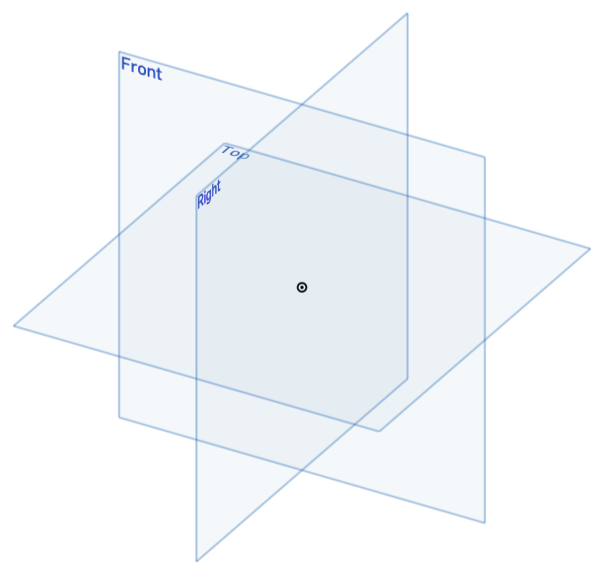
\includegraphics[width=5in]{figs/chap01_planes.png}}
\caption{Default planes intersecting at the origin.}
\label{chap01_planes}
\end{figure}

Planes are two-dimensional (2-D) slices through 3-D
space. All new parts in Onshape, like most CAD platforms
have the three planes, Top, Right, and Front. These
three planes are orthogonal, forming right angles
with each other and intersecting at the origin.

With the exception of motion simulations, gravity has no role in part development. This means that the Top, Right,and Front planes are equivalent, and parts can be developed in any orientation. All 2-D sketches must exist on a plane.

\index{planes}

\section{Moving and Selecting}
You can manipulate the workspace using the following 
mouse commands:

\begin{description}
\item[Zoom] with the scroll wheel.
\item[Rotate] by clicking the right mouse button and moving.
\item[Pan] by clicking the scroll wheel and moving.
Alternatively, you can hold 
\end{description}

Select a feature by clicking on it. Onshape uses persistent seletion, meaning that when you click on a second item, the first item remains selected, as in Figure \ref{chap01_selection}. The cursor tells you that two items are selected, and the {\bf feature tree} highlights which items those are. Deselect a single item by clicking it again. Deselect all items with the \keystroke{spacebar} or by clicking into empty space.

\begin{figure}[ht!]
\centerline{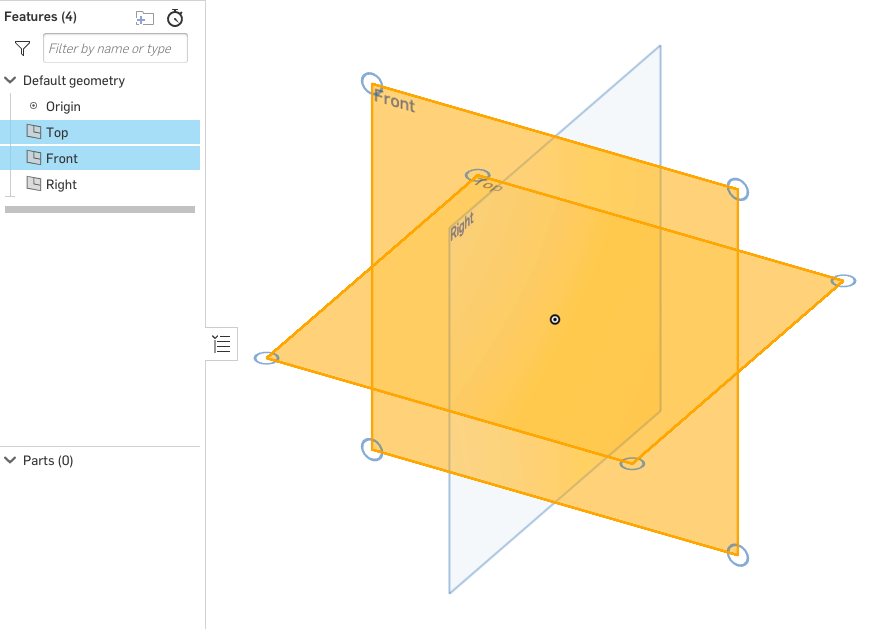
\includegraphics[width=5in]{figs/chap01_selection.png}}
\caption{Select multiple items by clicking on each. The feature tree (left) indicates which items are selected.}
\label{chap01_selection}
\end{figure}

\section{Sketches, Features, \& Models}
{\bf Sketches} provide two-dimensional geometry that act as the building block for three-dimensional parts. All sketches live on a plane. 

{\bf Features} turn two-dimensional sketches into three-dimensional solids and, less frequently, surfaces. Features often modify existing solids through Boolean operations such as addition, subtraction, or intersection.

{\bf Models}, also called parts, are the accumulation of three-dimensional features. Most models are {\bf solid models}, meaning that all features have thickness.
In contrast, {\bf surface models} have sketches and features but zero thickness. Like solid bodies, they are also the combination of multiple features.

Because sketches define two of the three dimensions of a feature, sketches capture the more detailed profile, and features extend that profile through space. If you were to CAD your hand, you might start with a sketch outlining your five fingers and palm, like the child's art project. Selecting the proper sketch profile builds a strong foundation for the rest of your model.

\section{The First Part}
As there is no traditional \href{https://en.wikipedia.org/wiki/%22Hello,_World!%22_program}{Hello World}
CAD part, I've elected that we'll make a triangular prism.

Start by selecting a single plane. Choose ``Sketch'' from the Feature Toolbar (\keystroke{shift} \keystroke{s}) to begin your sketch on that plane. 

It is often easier to sketch while viewing directly at, or normal to the plane. You can change your view by clicking on the View Cube, <right-click>-``View normal to'', or \keystroke{n}. I also prefer to toggle plane visibility off with the eyeball.

\begin{figure}[ht!]
\centerline{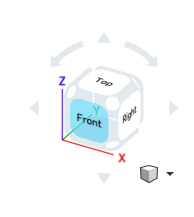
\includegraphics[width=3in]{figs/chap01_view_cube.png}}
\caption{The View Cube allows you to view models from pre-defined views.}
\label{view_cube}
\end{figure}

Sketch a right triangle with one leg vertical and one leg horizontal, both meeting at the origin, as in Figure \ref{start_sketch}. The two legs of the triangle are now black, meaning that they are {\bf constrained}. This means they are fully defined, and if you try to drag them, they will not move.

\begin{figure}[ht!]
\centerline{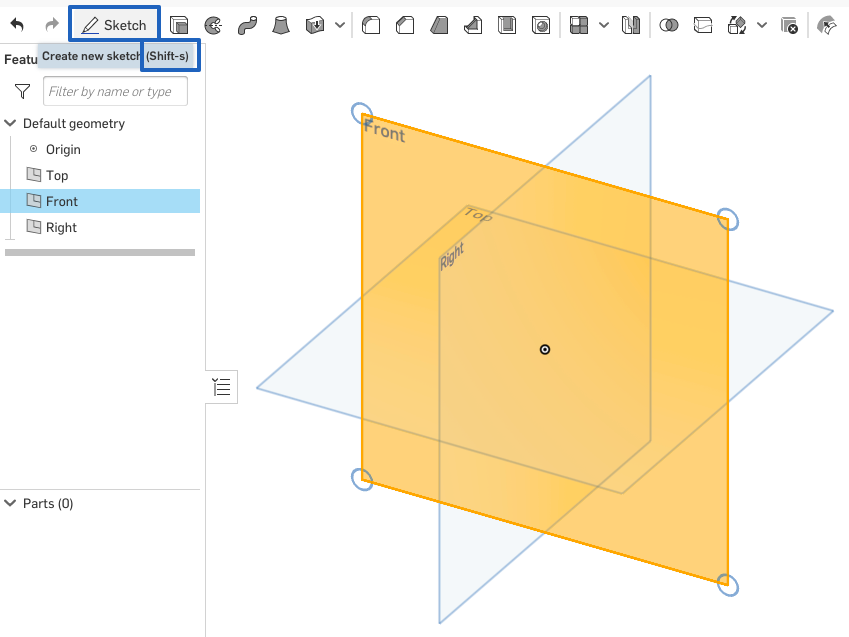
\includegraphics[width=4in]{figs/chap01_start_sketch.png}}
\caption{}
\label{}
\end{figure}

Note that the hypotenuse and each of its endpoints are blue, indicating that they are {\bf underconstrained}. Notice that endpoints move differently from edges when dragged. As sketches increase in complexity, it can be challenging to determine which degrees of freedom remain undefined. Dragging blue sketch entities can help you to understand where constraints are needed.

Constrain the sketch by adding a dimension (\keystroke{d}) of to one of the legs. Often, we'll want two dimensions to share the same size. We could accomplish this in a few ways.

\begin{description}
\item[Dimension both] - This is not preferable because changing
\end{description}

\section{Design Intent}
A key feature of well-done CAD is that it captures {\bf design intent}.

\section{Exercises}
\begin{exercise}
Locate the Onshape documentation on the extrude feature. Review the documentation for the desktop platform. Is it easier to access this documentation from the Onshape Help menu or from a search engine?
This will also be your first introduction to the Onshape mobile platforms, which won't be covered in this book.
\end{exercise}

\begin{exercise}
Modify your part to test additional options within Extrude. You might try these:

\begin{itemize}
\item Create a second closed shape within your triangle and extrude the first shape, second shape, both, or regions where they intersect.

\item Create a sketch on one of the faces of the first part. Extrude that sketch into or away from the prism, or in both directions. Test the ``New'', ``Add'', ``Remove'', and ``Intersect'' features. With each test, observe how many parts result in the Parts Tree.

\end{itemize}
\end{exercise}

\begin{exercise}
Delete constraints in your sketch until the sketch is underconstrained. Which ways are you able to move the sketch? Now constrain the sketch in different types of triangles, such as an equilateral. Can you make an isoceles triangle with a height that is twice the length of the base? Without equations?
\end{exercise}

\begin{exercise}
Change the first extrude to a surface rather than a solid. What happens when you try to add a solid body to a surface? What happens when you try to measure the thickness of one of the surfaces?
\end{exercise}
